\documentclass[tikz]{standalone}
\usepackage{pgfplots}
\pgfplotsset{compat=1.15}
\usepackage{mathrsfs}
\usetikzlibrary{arrows,calc}
\usepackage{tkz-euclide}
\pagestyle{empty}

\definecolor{AngleClr}{rgb}{0,0.39215686274509803,0}
\definecolor{ShapeClr}{rgb}{0.6,0.2,0}

\begin{document}

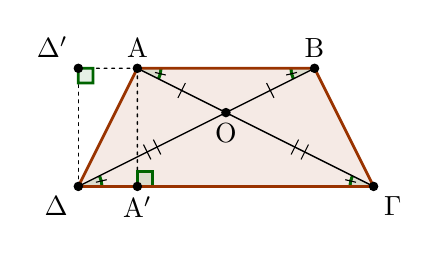
\begin{tikzpicture}[scale=.75]
\tkzSetUpLine[line width=1pt,color=black]
\tkzSetUpPoint[fill=black]

\tkzDefPoints{0/0/D,5/0/C,1/2/A,4/2/B}

\tkzDefPointBy[projection=onto C--D](A)\tkzGetPoint{A'}
\tkzDefPointBy[projection=onto A--B](D)\tkzGetPoint{D'}
\tkzInterLL(A,C)(B,D) \tkzGetPoint{O}

\tkzFillPolygon[fill=ShapeClr,fill opacity=0.1,inner sep=1cm](A,B,C,D)

\tkzDrawSegments[line width=0.5pt,color=black,dashed,dash pattern=on 1pt off 1.75pt](A,A' D,D' A,D')

\tkzMarkRightAngles[line width=1pt, size=.25,color=AngleClr,fill=AngleClr,fill opacity=0.1](A,A',C D,D',A)

\tkzFillAngles[fill=AngleClr,size=.4,fill opacity=0.1](A,B,D A,C,D C,A,B C,D,B)
\tkzMarkAngles[line width=1pt,color=AngleClr,size=.4](A,B,D A,C,D C,A,B C,D,B)
\tkzMarkAngles[mark=|,mksize=2,line width=1pt,size=.4,color=AngleClr](A,B,D A,C,D C,A,B C,D,B)

\tkzDrawSegments[line width=0.5pt,color=black](A,C B,D)

\tkzDrawPolygon[color=ShapeClr](A,B,C,D)
\tkzDrawPoints[size=3](A,B,C,D,A',D',O)
\tkzLabelPoint[above](A){$\rm A$}
\tkzLabelPoint[above](B){$\rm B$}
\tkzLabelPoint[below right](C){$\rm \Gamma$}
\tkzLabelPoint[below left](D){$\rm \Delta$}
\tkzLabelPoint[below](A'){$\rm A'$}
\tkzLabelPoint[above left](D'){$\rm \Delta'$}
\tkzLabelPoint[below](O){$\rm O$}

\tkzMarkSegments[mark=|,size=3](A,O B,O)
\tkzMarkSegments[mark=||,size=3](C,O D,O)

\end{tikzpicture}

\end{document}
